\documentclass[
  aspectratio=1610,
]{beamer}

\usepackage[american]{babel}
\usepackage[utf8]{inputenc}
\usepackage[T1]{fontenc}

% needs https://tex.stackexchange.com/questions/423848/xelatex-xy-and-dejavu-otf#423854
%\usepackage{dejavu-otf} % default Makie font: DejaVu Sans
%\usefonttheme{professionalfonts}

\title{A Low-Rank Parareal Solver for\\ Differential Riccati Equations\\ Written in Julia}
\author{Jonas Schulze}
\institute{Faculty of Mathematics\\ Otto-von-Guericke-Universität Magdeburg}
\date{May 10, 2022}
\subject{subject}

% beamer appearance
\setbeamercolor{block body}{bg=mpi} % for debugging
\setbeamercovered{transparent}
\beamertemplatenavigationsymbolsempty

\newcommand\maketocframe[1][]{%
  \begin{frame}{Outline}
    \tableofcontents[#1]
  \end{frame}
}

\AtBeginSection{%
  \maketocframe[currentsection,currentsubsection]
}

\usepackage[
  style=authoryear,
]{biblatex}
\addbibresource{stuff.bib}

\usepackage{mathtools}
\usepackage{xparse,xspace}
\usepackage{booktabs}
\usepackage{csquotes}
\usepackage[shortcuts]{glossaries}
\usepackage[binary-units]{siunitx}
\usepackage{listings}

\lstset{
  basicstyle=\small\ttfamily\color{black!15}, % should match transparency of covered
  columns=flexible,
}

\usepackage{tikz}
\usetikzlibrary{positioning}
\usetikzlibrary{graphs,arrows.meta}
\tikzset{>=Stealth}

\sisetup{
  round-mode = places,
  round-precision = 2,
}

\newcommand{\N}{\mathbb{N}} % Natural numbers
\newcommand{\Z}{\mathbb{Z}} % Whole numbers
\newcommand{\Q}{\mathbb{Q}} % Rational numbers
\newcommand{\R}{\mathbb{R}} % Real numbers
\newcommand{\C}{\mathbb{C}} % Complex numbers
\newcommand{\F}{\mathbb{F}} % Arbitrary Field
\newcommand{\K}{\mathbb{K}} % Arbitrary Field

\newcommand{\Cneg}{\C_-} % Negative Half Plane

\newcommand{\im}{i} % imaginary unit

\newcommand{\onehalf}{\tfrac{1}{2}}

% matrices
\newcommand\Cnn{\C^{n\times n}}
\newcommand\Rnn{\R^{n\times n}}
\newcommand\Rnr{\R^{n\times r}}
\newcommand\Rnk{\R^{n\times k}}
\newcommand\Rkk{\R^{k\times k}}
\newcommand\nnz{\operatorname{nnz}}
\renewcommand\vec{\operatorname{vec}}
\DeclareMathOperator{\colspan}{span}
\DeclareMathOperator{\orth}{orth}
\DeclareMathOperator{\rank}{rank}
\DeclareMathOperator{\diag}{diag}
\newcommand\MP{\dagger} % Moore Penrose pseudo-inverse

% transpose and conjugate/Hermitian transpose:
\newcommand\conj[1]{\overline{\optional{#1}}}
\newcommand\T{T}
\newcommand\HT{H}

% Rosenbrock
\newcommand\Ham{\ensuremath{H}}
\newcommand\Ricc{\operatorname{\mathcal R}}
\newcommand\Jac{\operatorname{\mathcal J}}

 % ADI
\newcommand\Aip{\mathop{H_k^+}}
\newcommand\Aim{\mathop{H_k^-}}
\newcommand\Aipm{\mathop{H_k^\pm}}
\newcommand\Aiip{\mathop{V_k^+}}
\newcommand\Aiim{\mathop{V_k^-}}
\newcommand\Aiipm{\mathop{V_k^\pm}}
\newcommand\Cayley{\mathop{\mathcal{C}}}
\newcommand\Aipinv{\mathop{(\Aip)^{-1}}}
\newcommand\Aiipinv{\mathop{(\Aiip)^{-1}}}
\newcommand\Lyap{\operatorname{\mathcal L}}

% usage: \{2x\given x\in\N}
\newcommand{\given}{\mid}

% usage: \Set[\big]{2x \given x\in\N}
\newcommand\SetSymbol[1][]{%
  \nonscript\:#1\vert
  \allowbreak
  \nonscript\:
  \mathopen{}}
\DeclarePairedDelimiterX{\Set}[1]{\lbrace}{\rbrace}{%
  \renewcommand\given{\SetSymbol[\delimsize]}% this effect is local only
  #1%
}

% personal taste:
\let\epsilon\varepsilon
%\renewcommand{\to}{\longrightarrow}
%\renewcommand{\mapsto}{\longmapsto}
%\renewcommand{\gets}{\longleftarrow}
\renewcommand{\Re}{\operatorname{Re}} % real part of a complex number
\renewcommand{\Im}{\operatorname{Im}} % imaginary part

% some more delimiters:
\NewDocumentCommand{\optional}{m}{\ifblank{#1}{\,\cdot\,}{#1}}
\DeclarePairedDelimiterX{\abs}[1]{\lvert}{\rvert}{\optional{#1}}
\DeclarePairedDelimiterX{\norm}[1]{\lVert}{\rVert}{\optional{#1}}
\DeclarePairedDelimiterX{\scalar}[2]{\langle}{\rangle}{\optional{#1},\optional{#2}}
\newcommand{\card}{\abs}

% integration:
\NewDocumentCommand{\intd}{m}{\,\textup{d}#1}
\newcommand\dt{\intd{t}}

% differentiation:
\NewDocumentCommand{\pdiff}{mm}{\frac{\partial #2}{\partial #1}}
\NewDocumentCommand{\diff}{mm}{\frac{\mathrm{d} #2}{\mathrm{d} #1}}

\newcommand\julia\texttt
\newcommand\code\texttt

\newcommand\LDLt{LDL\textsuperscript{T}}

\counterwithout*{footnote}{chapter}
\setcounter{topnumber}{1} % max number of floats at top of page
\renewcommand{\bottomfraction}{0.5}
\renewcommand{\listtheoremname}{List of Theorems and Examples}

\newcommand\LandauO{\operatorname{\mathcal O}}

% runtime estimates
\newcommand\hattpar{\hat t_\text{par}} % estimate
\newcommand\hattseq{\hat t_\text{seq}} % estimate
\newcommand\tpar{t_\text{par}}
\newcommand\tseq{t_\text{seq}}
\newcommand\twarmup{t_\text{warm-up}}
\newcommand\trampup{t_\text{ramp-up}}
\newcommand\JIT{\operatorname{compile}}

% error estimates
\newcommand\umach{\mathrm u_\text{mach}} % machine precision

% https://tex.stackexchange.com/questions/22561/what-is-the-proper-use-of-i-e-backslash-at?noredirect=1&lq=1
\makeatletter % no idea why this is needed. \@ifnextchar doesn't work without it.
\newcommand\cf{cf.\@\xspace} % confer
\newcommand\eg{e.g.\@\xspace} % exempli gratia
\newcommand\etc{etc\@ifnextchar.{}{.\@\xspace}} % et cetera
\newcommand\ie{i.e.\@\xspace} % id est
\newcommand\wrt{w.r.t.\@\xspace} % with respect to
\makeatother

\definecolor{mathcore} {RGB}{102,  99, 100}
\definecolor{ovgu math}{RGB}{209,  63,  88}
\definecolor{mpi}      {RGB}{ 61, 167, 197}
\def\cola{ovgu math}
\def\colb{mathcore}
\def\colc{mpi}

\tikzset{
  mat/.style={
    rectangle,
    minimum size=1ex,
    inner sep=0mm,
  },
  bigmat/.style={mat,minimum size=#1},
  bigmat/.default=1cm,
  tallmat/.style={mat,minimum height=#1},
  tallmat/.default=1cm,
  widemat/.style={mat,minimum width=#1},
  widemat/.default=1cm,
  smallmat/.style={mat},
}

\newcommand\mat[2]{%
  \tikz[baseline=(M.base)] \node [mat, #1, fill=ovgu math] (M) {$#2$};
}
\newcommand\bigmat[1]{\mat{minimum size=2cm}{#1}}
\newcommand\tallmat[2][6mm]{\mat{minimum size=#1, minimum height=2cm}{#2}}
\newcommand\widemat[2][6mm]{\mat{minimum size=#1, minimum width=2cm}{#2}}
\newcommand\smallmat[2][6mm]{\mat{minimum size=#1}{#2}}

\newcommand\tallcmat[1]{\tikz[baseline=-0.5ex]\node[tallmat,fill=#1] {};}
\newcommand\smallcmat[1]{\tikz\node[smallmat,fill=#1] {};}
\newcommand\widecmat[1]{\tikz\node[widemat,fill=#1] {};}
\newcommand\colorldlt[1]{%
  \mathop{\tallcmat{#1}}
  \mathop{\smallcmat{#1}}
  \mathop{\widecmat{#1}}
}

\newcommand\colorspacing{%
  \arraycolsep=3pt
  \def\arraystretch{0.75}
}


\begin{document}

\frame[plain]{\titlepage}
\maketocframe

\section{Motivation}

\everymath{\displaystyle}

\begin{frame}{Motivation}
  \begin{columns}[t,onlytextwidth]
  \column{0.5\linewidth}
  \begin{block}{\strut Optimal Control Problem}
    Consider the \ac{LQR} problem
    \begin{equation*}
      \begin{array}{cl}
        \min_u & \int_{t_0}^{t_f} y^\T y + u^\T u \dt + \tfrac{1}{100} y(t_f)^\T y(t_f) \medskip\\
        \text{s.t.} & \begin{aligned}[t]
          E \dot x &= Ax + Bu \\
          y &= Cx
        \end{aligned}
      \end{array}
    \end{equation*}
    using
    \begin{itemize}
      \item
        state $x(t)\in\R^n$
      \item
        control $u(t)\in\R^m$, $m\ll n$
      \item
        output $y(t)\in\R^q$, $q\ll n$
      \item
        autonomous system matrices $E, A \in\Rnn$, $B\in\R^{n\times m}$, $C\in\R^{q\times n}$
    \end{itemize}
  \end{block}
  \column{0.45\linewidth}
  \begin{block}{\strut Feedback Law}
    The optimal control is given by
    \begin{equation*}
      u(t) = - \underbrace{
        B^\T X(t) E
      }_{
        K\mathrlap{(t)}
      }
      x(t)
    \end{equation*}
    where $X(t)\in\R^{n\times n}$ solves the \ac{DRE}
    \begin{equation*}
      \left\{
        \begin{aligned}
          E\dot X E &= C^\T C + A^\T X E + E^\T X A - E^\T X BB^\T X E \\
          E^\T X(t_0) E &= \tfrac{1}{100} C^\T C
        \end{aligned}
      \right.
    \end{equation*}
  \end{block}
  \end{columns}
\end{frame}

\begin{frame}
  \begin{itemize}
    \item
      For a resolution of \SI{1}{\milli\second} along $[t_0,t_f] = [0, \SI{45}{\second}]$,
      storing $X$ takes ... memory

      $\leadsto$ only store $K := B^\T X E$
    \item
      For moderate size $n=\num{20000}$, a single (dense) $X(t)\in\Rnn$ takes \SI{3.2}{\giga\byte}.

      But: solution usually has low numerical rank \\
      \parencite[e.g.][]{Lang2017,Kuerschner2016,Penzl2000}

      $\leadsto$ \ac{LRSIF}
      \begin{equation}
        \bigmat{X} = \mathop{\tallmat{L}} \mathop{\smallmat{D}} \mathop{\widemat{L^{\smash{\T}}}}
      \end{equation}
    \item
      For a resolution of \SI{1}{\milli\second} along $[t_0,t_f] = [0, \SI{45}{\second}]$,
      and small $n=371$,
      computing a 4th order trajectory sequentially takes about 1 day.

      $\leadsto$ need further parallelization
  \end{itemize}
\end{frame}

\newcommand\tallcmat[1]{\tikz[baseline=-0.5ex]\node[tallmat,fill=#1] {};}
\newcommand\smallcmat[1]{\tikz\node[smallmat,fill=#1] {};}
\newcommand\widecmat[1]{\tikz\node[widemat,fill=#1] {};}
\newcommand\colorldlt[1]{%
  \mathop{\tallcmat{#1}}
  \mathop{\smallcmat{#1}}
  \mathop{\widecmat{#1}}
}

\newcommand\colorspacing{%
  \arraycolsep=3pt
  \def\arraystretch{0.75}
}

\begin{frame}{Low-Rank Symmetric Indefinite Factorization}
  \begin{itemize}
    \item \cite{Benner2009}
    \item Addition/Subtraction:
      \begin{equation*}
        \colorspacing
        \colorldlt{\cola} \pm \colorldlt{\colc}
        :=
        \Bigg[
        \begin{matrix}
          \tallcmat{\cola} &
          \tallcmat{\colc}
        \end{matrix}
        \Bigg]
        \begin{bmatrix}
          \smallcmat{\cola} \\
          & \pm \smallcmat{\colc}
        \end{bmatrix}
        % flag of the Netherlands:
        \begin{bmatrix}
          \widecmat{\cola} \\
          \widecmat{\colc}
        \end{bmatrix}
      \end{equation*}
    \item Problem: growing rank
      \begin{equation*}
        \colorspacing
        \colorldlt{\cola} + \colorldlt{\cola}
        :=
        \Bigg[
        \begin{matrix}
          \tallcmat{\cola} &
          \tallcmat{\cola}
        \end{matrix}
        \Bigg]
        \begin{bmatrix}
          \smallcmat{\cola} \\
          & \smallcmat{\cola}
        \end{bmatrix}
        % flag of Austria:
        \begin{bmatrix}
          \widecmat{\cola} \\
          \widecmat{\cola}
        \end{bmatrix}
        %\not\equiv
        %\mathop{\tallcmat{\cola}}
        %\mathop{(\smallcmat{\cola} + \smallcmat{\cola})}
        %\mathop{\widecmat{\cola}}
      \end{equation*}
      $\leadsto$ Column compression techniques
  \end{itemize}
\end{frame}

\begin{frame}
  \begin{block}{Parareal Method \parencite{Lions2001}}
    \begin{equation*}
      \left\{
      \begin{aligned}
        U^0_{n+1} &:= G(U^0_n) \\
        U^{k+1}_{n+1} &:= G(U^{k+1}_n) + F(U^k_n) - G(U^k_n)
      \end{aligned}
      \right.
    \end{equation*}
  \end{block}
  in low-rank formulation:
  \begin{equation*}
    \colorspacing
    U^{k+1}_{n+1}
    = \underbrace{\colorldlt{\cola}}_{G(U^{k+1}_n)}
    + \underbrace{\colorldlt{\colb}}_{F(U^{k}_n)}
    - \underbrace{\colorldlt{\colc}}_{G(U^{k}_n)}
    =
    \Bigg[
    \begin{matrix}
      \tallcmat{\cola} &
      \tallcmat{\colb} &
      \tallcmat{\colc}
    \end{matrix}
    \Bigg]
    \begin{bmatrix}
      \smallcmat{\cola} \\
      & \smallcmat{\colb} \\
      && -\smallcmat{\colc}
    \end{bmatrix}
    \begin{bmatrix}
      \widecmat{\cola} \\
      \widecmat{\colb} \\
      \widecmat{\colc}
    \end{bmatrix}
  \end{equation*}
\end{frame}

\section{Results}

\begin{frame}
  \frametitle{Results}
  foo
\end{frame}

\section{Summary}

\begin{frame}
  \frametitle{Summary}
  foo
\end{frame}

\appendix

\begin{frame}
  table 7.3
\end{frame}

\renewcommand\mathrm\mathsf % fix \umach
\newcommand\sidenote[1]{\footnotesize{\textcolor{gray}{#1}}}

\begin{frame}[fragile]
  \frametitle{Parareal Reference Solution}
  \begin{itemize}
    \item
      Thesis Figure 7.7: parareal order 4/4

      \begin{lstlisting}
MY_KIND=dense MY_NF=100 MY_OF=4 MY_OC=4 sbatch -n450 -c1 -J de44 par.job
      \end{lstlisting}
      %MY_NF=100 MY_OF=4 MY_OC=4 sbatch -pmedium --time=2:00:00 -n 450 -c1 -J d44 dense-par.job
    \item
      Better: sequential order 4

      \begin{lstlisting}
MY_KIND=dense MY_N=45000 MY_O=4 sbatch -n1 -c1 -J de4 seq.job
      \end{lstlisting}
      % MY_N=45000 MY_KIND=dense MY_O=4 sbatch --partition=long --time=2-00:00:00 -n1 -c1 -J de4-c1 seq.job
    \item
      Relative error negligible:
      \begin{equation*}
        \frac{\norm{K_\text{par}(t) - K_\text{seq}(t)}_F}{\norm{K_\text{seq}(t)}_F}
        < 5\umach
      \end{equation*}
  \end{itemize}
\end{frame}

\begin{frame}
  \frametitle{Relative Error of Parareal Reference Solution}
  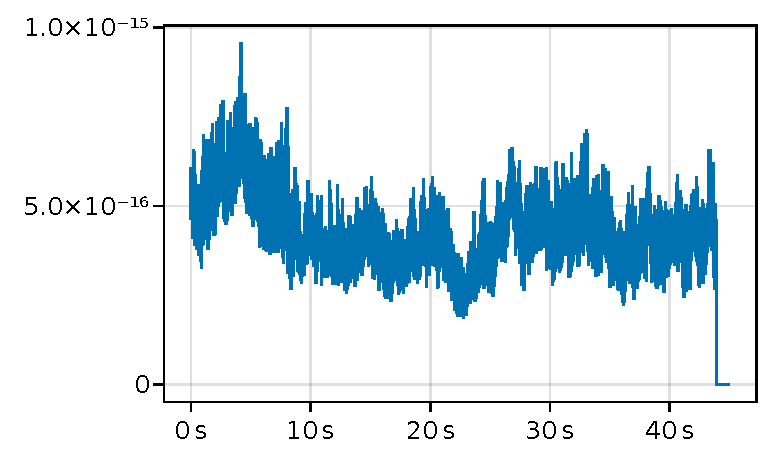
\includegraphics[width=0.8\textwidth]{figures/slides-seq-parareal-ref.pdf}
\end{frame}

\end{document}
